
%%%%%%%%%%%%%%%%%%%%%%%%%%%%%%%%%%%%%%%%%%%%%%%%%%%%%%%%%%%%%%%%%%%%%%%%%%%%%%%%
\section{Introduction}
Creative solutions are necessary to meet the \gls{SNF} disposal challenges 
faced by the United States.
This work proposes and evaluates a strategy that leverages the 
remaining resources inherent in a shut down nuclear reactor site toward a new 
purpose: a consolidated interim storage and spent fuel repository facility.

Domestic nuclear power plants are at risk of shutdown in areas with surplus 
electricity capacity from coal and new natural gas. Kewaunee and Crystal River 
have already closed  and numerous other plants are at risk in the near term 
\cite{nei_nuclear_2014}.  Simultaneously, the \gls{DOE} 
has begun to move forward with consent-based siting of a nuclear 
spent fuel repository \cite{doe_designing_2016}. The proposed solution in this 
work seeks to combine these efforts toward a more economic and politically 
feasible solution. 

% explain that this work compares the base case with the proposal
This work compares a base case which is to site a borehole-type repository in the
 Yucca Mountain region, to a base case, which is to site a borehole-type repository
 next to a shutdown nuclear power plant. The main expected benefits arising from the
 proposed case is transportation burden of radioactive waste, more consent-based
 siting with the local community, and modularity of the repository. 

% note the metrics on which these two cases are being compared.
Each incentive criteria in the comparison is given a numerical value, which is
weighted to its importance to various stakeholders. 

\subsection{Motivation}
The proposed integrated siting strategy takes advantage of three technical 
benefits of borehole repository designs: modularity, broad geological 
suitability, and footprint efficiency. Modularity enables regional repositories 
to scale in size according to the local spent fuel burden. 
Additionally, the necessary geological characteristics required for borehole 
disposal, crystalline basement rocks at $2,000 m - 5,000 m$ deep, are relatively 
common in stable continental regions \cite{arnold_research_2012}. Finally, the 
surface footprint requirements of a borehole repository are comparable to the 
available footprint of a nuclear power reactor site, with only $30 km^2$ 
required for the total \gls{SNF} amount proposed for Yucca Mountain 
\cite{brady_deep_2009}.

Integrated siting also has potential economic benefits. One significant cost 
inherent to borehole repository concepts is the repacking of spent fuel 
assemblies into smaller-diameter waste canisters representing over 15\% of 
estimated per-borehole cost \cite{arnold_reference_2011}.  However, siting a 
repository at a non-operating power plant facility, especially one with a 
dry-cask storage site, will take advantage of already existing infrastructure 
and local human talent for spent fuel handling and packaging. Many candidate 
non-operating reactor sites, such as those mapped in Figure \ref{fig:shutdown}, 
may be appropriate for integrated siting if they are located above crystalline 
basement formations and include dry cask packaging facilities.

Finally, integrated siting may be more practically and politically feasible. 
Preliminary work \cite{waleed_regional_2015} indicates integrated siting is 
appealing to many stakeholder groups. For example, a consent-based approval 
process may be feasible because communities local to power plants may be 
uniquely receptive to the incentives of hosting a repository.  

%%%%%%%%%%%%%%%%%%%%%%%%%%%%%%%%%%%%%%%%%%%%%%%%%%%%%%%%%%%%%%%%%%%%%%%%%%%%%%%

\section{Methodology}

This work will evaluate the potential impacts of integrated siting from the 
perspective of 5 stakeholders:
\begin{itemize}
        \item the federal government,
        \item the state government,
        \item the local government,
        \item the local community,
        \item and the owner of the non-operating plant.
\end{itemize}


Preliminary work \cite{waleed_regional_2015} suggests that integrated siting 
will reduce costs, construction, time (both for construction and licensing), 
transportation distances, and resistence from the local community.  The present 
work will compare the proposal along these axes to a base case: a standalone 
borehole repository at a similar location to that of Yucca Mountain.  
Quantification of those stakeholder benefits will be undertaken for two 
different regions of the US in addition to the base case.  

The goal of this paper is to compare this siting strategy with the 
business-as-usual base case via quantitative metrics capturing the key 
priorities of stakeholders. 

\begin{figure}[!h] 
  \centering
  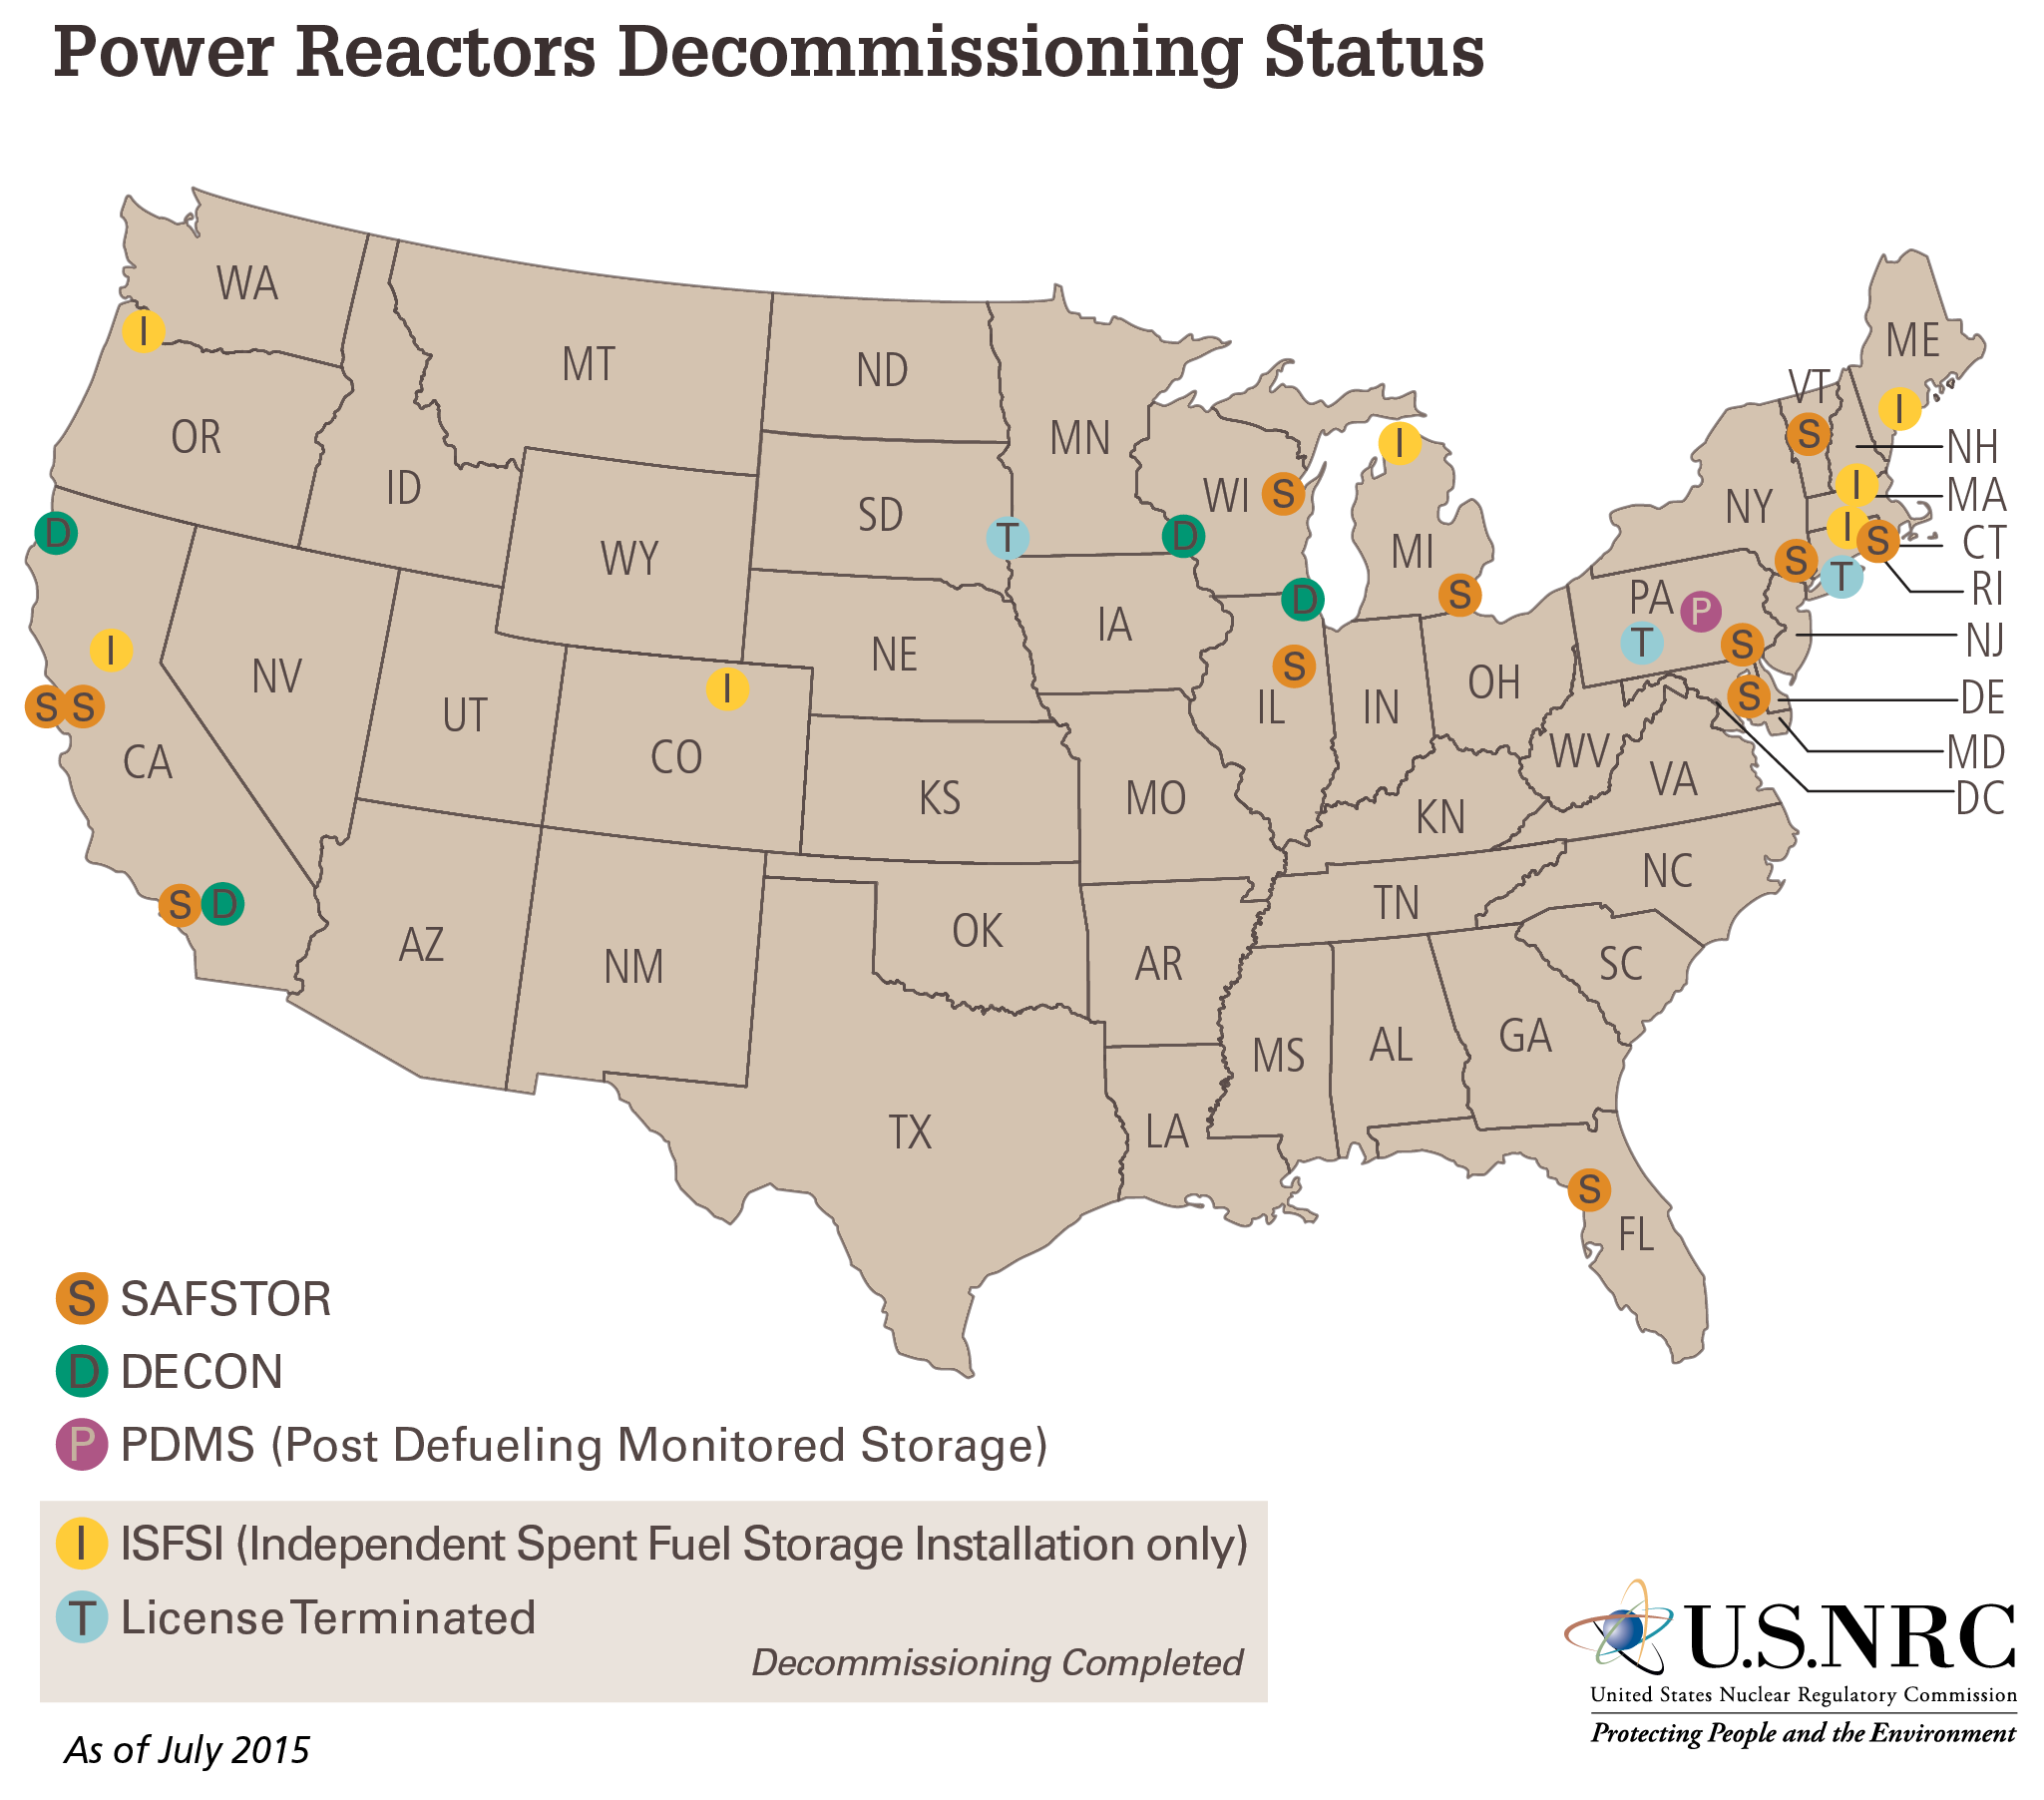
\includegraphics[width=0.8\columnwidth]{power-reactors-decommissioning}	
  \caption{Non-operating facilities status
  \cite{nuclear_regulatory_commission_nrc_2015}.}
  \label{fig:shutdown}
\end{figure}


